%---------- Inleiding ---------------------------------------------------------

\section{Introductie} % The \section*{} command stops section numbering
\label{sec:introductie}

De Vlaamse Overheid investeert in het Vlaamse cultureel erfgoed door collectiebeherende instellingen te ondersteunen en kwaliteitslabels uit te reiken. In ruil voor die steun verwacht de Vlaamse Overheid dat die instellingen een aantal taken uitvoeren, waaronder het registreren, inventariseren en metadateren van cultureel-erfgoedobjecten op een gestandaardiseerde manier, het onderzoeken (en faciliteren van onderzoek) en het presenteren van de collectie.~\autocites{AKE2014}{Gatz2016}

De collectiebeherende instellingen lijden aan een historische achterstand m.b.t. de registratie van de eigen collectie~\autocite{Gatz2016}. In 2018 werd daarom een nieuwe subsidielijn opgestart om de digitale collectieregistratie weg te werken. Deze subsidielijn werd opgestart vanuit de vaststelling dat de competenties en strategie{\"e}n ontbreken om een inhaalbeweging te realiseren~\autocite{JeugdMediaC2018a}.

In de bachelorproef willen we onderzoeken in welke mate Computer Vision API's (vanaf nu afgekort als CVA), zoals Google Cloud Vision\footnote{\url{https://cloud.google.com/vision/}} of Microsoft Computer Vision API\footnote{\url{https://azure.microsoft.com/nl-nl/services/cognitive-services/computer-vision/}}, ingezet kunnen worden om dit registratieproces te versnellen en als strategie gebruikt kunnen worden om een inhaalbeweging te realiseren. Momenteel gebeuren registraties door domeinexperten. Dit is tijdrovend werk. Met behulp van artifici{\"e}le intelligentie (AI) kan dit proces deels geautomatiseerd worden. Dit geeft de collectieregistrator de mogelijkheid om zich met minder basaal werk bezig te houden en geeft de musea de kans hun collectie sneller te ontsluiten.

Het VKC Datahub Dashboard\footnote{\url{https://dashboard.vlaamsekunstcollectie.be}} geeft een goed beeld van de registratieachterstand in Vlaanderen. Dit dashboard analyseert de collectieregistratie van de Vlaamse musea voor Schone (en in de toekomst ook Hedendaagse) Kunsten die aangesloten zijn bij de VlaamseKunstCollectie (VKC)\footnote{\url{http://vlaamsekunstcollectie.be/}}, waaronder het aantal records ingevuld volgens de minimale registratie en het aantal records ingevuld volgens de basisregistratie.\footnote{De minimale registratie omvat de elementen en velden die in overeenstemming met de ICOM Code of Ethics minimaal gedocumenteerd moeten worden wanneer een object een museum binnenkomt: d.i. bewaarinstelling, objectnummer, titel, korte beschrijving, objectnaam, verwervingsmethode, verwervingsbron en verwervingsdatum. De velden voor de basisregistratie bevatten de acht velden voor minimale registratie en voegen hier nog een tiental andere velden aan toe. Voor meer info, zie het \href{https://www.projectcest.be/wiki/Publicatie:Invulboek_objecten/Profielen/Basisregistratie}{Invulboek Objecten op CEST}} Dit zijn cijfers van de grooste kunstmusea van Vlaanderen. Uit de cijfers blijkt dat vooral formele en administratieve gegevens geregistreerd worden; inhoudelijke informatie, zoals afgebeelde persoon of afgebeeld concept, die interessant is voor ontsluiting en onderzoek, ontbreekt hoofdzakelijk.

\begin{figure}[h]
	\caption{Het overzicht van de velden van de basisregistratie en het aantal keer dat ze aanwezig zijn in de collectiedata van MSK Gent.}
	\centering
	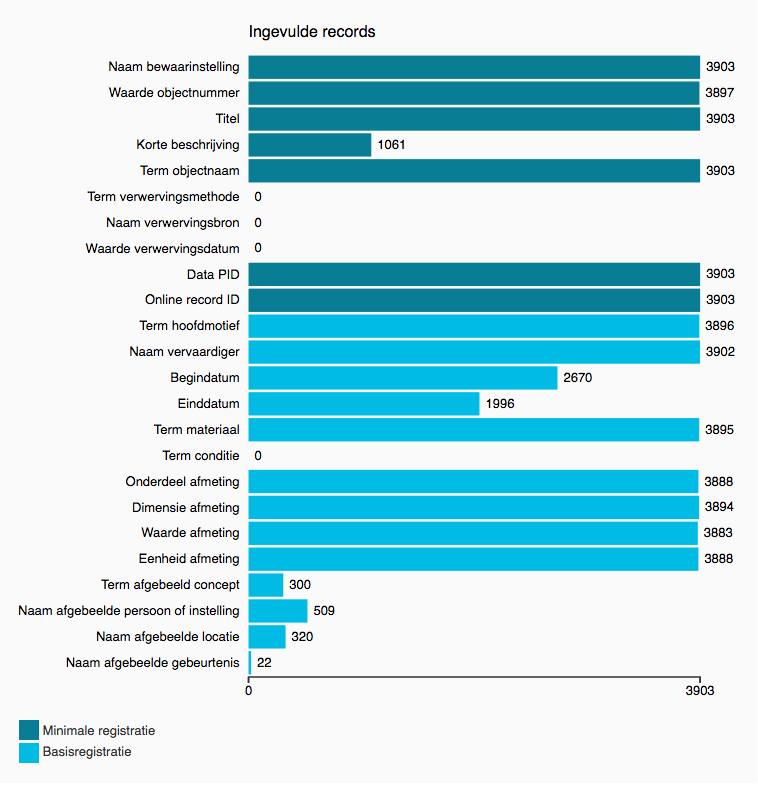
\includegraphics[width=\linewidth]{/Users/nastasiavanderperren/iCloud/Documents/Informatica_Hogent/BA3/bachelorproef/voorstel/pictures/VKC_velden_basis.png}
\end{figure}

In het verleden werd reeds (theoretisch) onderzoek verricht naar het gebruik van Computer Vision voor cultureel erfgoed en kunst.\footnote{Zie infra, in het deel \emph{Stand van zaken}.} De resultaten van dit onderzoek waren veelbelovend. Nieuwe ontwikkelingen zorgen ervoor dat Computer Vision steeds meer accuraat wordt en steeds eenvoudiger in gebruik, waardoor het meer en meer een instrument wordt waarmee ook developers aan de slag kunnen~\autocite{Hindle2017}.

%---------- Stand van zaken ---------------------------------------------------

\section{Stand van zaken}
\label{sec:state-of-the-art}

\subsection{Computer Vision en (cultureel) erfgoed}
Een aantal instellingen maken al gebruik van Computer Vision voor de ontsluiting van hun collectie:
\begin{itemize}
	\item \textbf{The Museum of Modern Art (MoMA)}\footnote{\url{https://www.moma.org/}} gebruikte diensten van Google via \emph{Google Arts Culture Lab} om aan de historische foto's van afgelopen tentoonstellingen in MOMA foto's uit de kunstcollectie te koppelen. Het algoritme analyseerde hiervoor alle foto's van tentoonstellingszichten. Als het een kunstwerk op de foto's kon herkennen, dan werd er een koppeling gelegd met de afbeelding van dit kunstwerk in de collectie van MOMA.\footnote{Bekijk een voorbeeld over \href{https://www.moma.org/calendar/exhibitions/1767/installation_images/10473}{een tentoonstelling over C\`{e}zanne, Gaugain, Seurat en Van Gogh uit 1929}} MOMA stelde hierbij vast dat het logaritme vooral goed scoort op het vlak van tweedimensionele, statische afbeeldingen (bv. een afbeelding van een kunstwerk), maar dat het minder goede resultaten geeft met afbeeldingen van 3D-objecten (bv. een standbeeld) of bewegend beeld~\autocite{MOMA2018?}.

	\item Het \textbf{Smithsonian}\footnote{\url{https://www.smithsonianmag.com/}} gebruikt AI-technologie om stalen van planten te classificeren. Het Smithsonian is gestart met het systematisch digitaliseren van de collectie voor wetenschappers en in functie van online ontsluiting. De AI-technologie slaagde erin om via deze afbeeldingen twee gelijkaardige planten te onderscheiden met een succesgraad van meer dan 90\%~\autocite{Smith2017}.

	\item Het \textbf{Nasjonalmuseet}\footnote{\url{http://www.nasjonalmuseet.no/en/}} was het onderwerp van het \emph{Principal Components} onderzoek. Hierbij werd met het deep learning framework Caffe\footnote{Voor meer info, zie: \url{http://caffe.berkeleyvision.org/}} gezocht naar compositionele gelijkenissen tussen kunstwerken en werden ze geclassificeerd op basis van de Iconclass-termen\footnote{Iconclass is een gespecialiseerd kunsthistorisch classiciatiesysteem, \url{https://nl.wikipedia.org/wiki/Iconclass}}. Dit resulteerde in een vernieuwende publiekstoegang tot de collectie waarbij de kunstwerken op basis van gelijkenissen gevisualiseerd werden. Hoe meer gelijkenissen, hoe dichter de kunstwerken bij elkaar staan.\footnote{\href{http://vy.nasjonalmuseet.no/?collection=painting_subject}{Bekijk bijvoorbeeld schilderijen op basis van hun motief}.} \autocites{Nasjonalmuseet2017?}{Westvang2017?}
\end{itemize}

\subsection{Theoretisch onderzoek}
Daarnaast is eerder theoretisch onderzoek gedaan naar het gebruik van Computer Vision binnen een erfgoedcontext. In onderstaande lijst worden de onderzoeken vermeld die zich focussen op museumcollecties:
\begin{itemize}
	\item \textbf{Using Machine Learning for Identification of Art Paintings (2013)}: In dit onderzoek werd machine learning gebruikt voor het classificeren van kunstwerken van zeven kunstenaars: C\'{e}zanne, Dali, D\"{u}rer, Monet, Picasso, Rembrandt en Van Gogh. Per kunstenaar werden er tweehonderd kunstwerken gezocht. In 87,13\% van de gevallen was de computer correct. De onderzoekers vermoedden dat dit resultaat nog beter kan zijn als de training set groter is.~\autocite{Blessings2013}

	\item \textbf{The Rijksmuseum Challenge: Museum-Centered Visual Recognition (2014)}: Beelden die publiek beschikbaar zijn via de API van Het Rijksmuseum\footnote{\url{https://www.rijksmuseum.nl/en/api}} werd gebruikt voor het oplossen van vier challenges:
	\begin{itemize}
		\item voorspel de kunstenaar van het afgebeelde object;
		\item voorspel het materiaal dat gebruikt werd voor het afgebeelde object;
		\item voorspel het jaar waarin het object gemaakt werd;
		\item voorspel het soort object (schilderij, tekening, standbeeld...) dat afgebeeld wordt.
	\end{itemize}
	Het ging om objecten die afkomstig waren van de oudheid tot de late 19e eeuw en om een veelheid aan objecten: schilderijen, foto's, keramiek, meubels, etc. Ook in dit onderzoek waren de resultaten veelbelovend.~\autocite{Mensink2014}

	\item \textbf{INSIGHT (2017-2020)}: Hier wil men onderzoeken hoe AI kan gebruikt worden om collecties uit de cultureel-erfgoedsector van beschrijvende metadata te voorzien. De collecties van de Koninklijke Musea voor Schone Kunsten van Belgi\"{e} en de Koninklijke Musea voor Kunst \& Geschiedenis worden als testcase gebruikt. De focus ligt op het vrijgeven van die data als open datasets.~\autocite{UniAntwerpen2017?} Uit de paper \emph{Deep Transfer Learning for Art Classification Problems} van \textcite{Sabatelli2018} kwamen veelbelovende resultaten naar boven voor het voorspellen van materiaal, objecttype en kunstenaar.

	\item \textbf{Automated Image Analysis with IIIF (2017)}: Dit onderzoek is eerder praktisch gericht en werd uitgevoerd buiten de academische wereld. Het werd uitgevoerd door CogApp, een bedrijf dat software ontwikkelt voor online archieven en musea.\footnote{\url{https://www.cogapp.com/about/}} Zij hebben verschillende testen gedaan met machine learning. Het meest interessant voor dit voorstel is het onderzoek waarbij drie Computer Vision API's (Google Cloud Vision, Microsoft Computer Vision en Clarifai\footnote{\url{https://www.clarifai.com/}}) getest werden om beelden te voorzien van extra tags om de doorzoekbaarheid te verbeteren. Naast de grappige resultaten~\autocite{Roddis2018}, leidde dit tot goede resultaten waarmee de beeldencollectie op een interessante manier doorzocht kan worden: Je kan er een selectie van beelden verkrijgen door te filteren op verschillende tags, bv. \emph{ik wil een kunstwerk uit de Renaissance van iemand met een snor en een cape}.\footnote{Probeer het zelf op: \url{http://labs.cogapp.com/iiif-ml/}} De onderzoekers concludeerden dat de CVA accurate beschrijvingen geven en dat Computer Vision steeds eenvoudiger in gebruik wordt. De foutieve beschrijvingen, zoals in Figuur 2, zijn vermoedelijk een gevolg van het trainen van CVA met hedendaagse beelden die gemaakt werden met een smartphone.~\autocite{Hindle2017}

	\begin{figure}[h]
		\caption{Vrouw en man met boek worden door Microsoft Computer Vision ge\"{i}dentificeerd als man en vrouw die een selfie nemen~\autocite{Roddis2018}.}
		\centering
		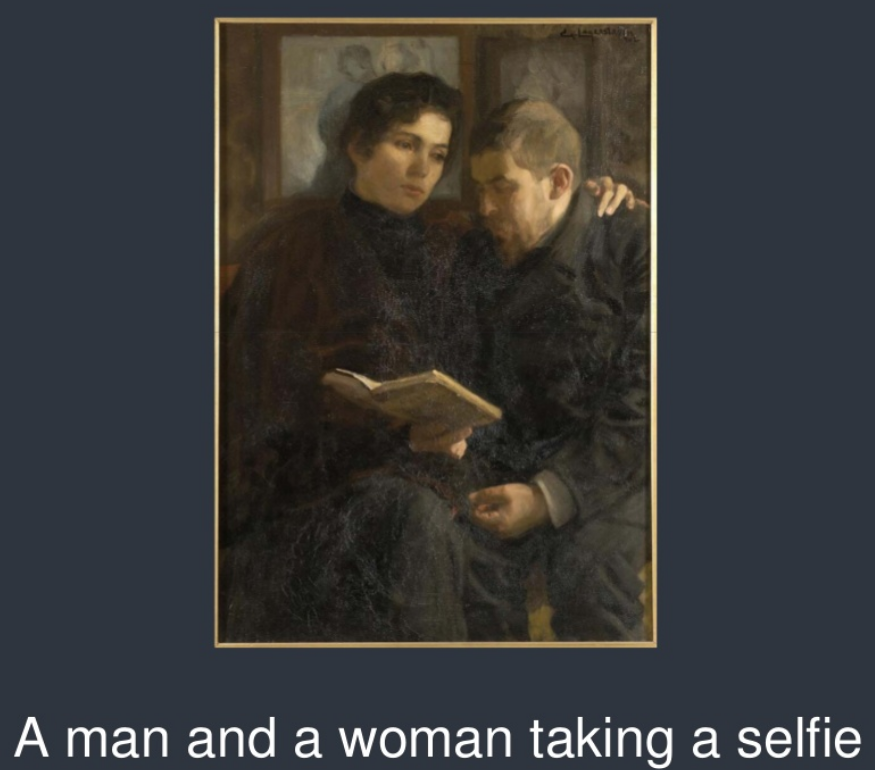
\includegraphics[width=\linewidth]{/Users/nastasiavanderperren/iCloud/Documents/Informatica_Hogent/BA3/bachelorproef/voorstel/pictures/roddis_grappig_2}
	\end{figure}

\end{itemize}

\subsection{Computer Vision API's}
Tot slot lichten we kort CVA toe. CVA, ook wel image/visual recognition API's genoemd, zijn API's die afbeeldingen automatisch kunnen taggen (metadateren), organiseren en zoeken via machine learning. Het biedt de mogelijkheid om machine learning toe te passen zonder dat je hier zelf een expert in moet zijn. Je kan er zelf modellen mee cre\"{e}ren om de API's te trainen naar je eigen behoefte. Zo leerde Matt Fraser Google Cloud Vision verschillende spinnen te herkennen door de dienst te trainen met honderd afbeeldingen per spin~\autocite{Fraser2018}.  De bekendste diensten zijn Clarifai, IBM Visual Recognition\footnote{\url{https://www.ibm.com/watson/services/visual-recognition/}}, Microsoft Computer Vision en Google Cloud Vision.  De diensten zijn zo toegankelijk dat iedere ontwikkelaar zonder machine learning kennis modellen kan bouwen, maar dat ook, volgens TechCrunch, iedereen zonder programmeerervaring de diensten kan gebruiken om afbeeldingen te taggen en categoriseren~\autocite{Lardinois2018}. Ook uit het onderzoek van CogApp bleken de diensten eenvoudig in gebruik en precies te trainen \autocite{Hindle2017}.

%---------- Methodologie ------------------------------------------------------
\section{Methodologie}
\label{sec:methodologie}

In dit onderzoek zal bestudeerd worden of CVA helpen bij het inhoudelijk ontsluiten van erfgoedcollecties. Kunnen de ingebouwde modellen van de API's gebruikt worden, of is er nood aan (doorgedreven) training? Dit wordt onderzocht aan de hand van een prototype waarmee verschillende beelden geanalyseerd worden. Hiervoor wordt een CVA gekozen die het toelaat om eigen modellen te trainen via een webinterface, voorzien is van goede documentatie en tutorials en beschikt over API clients in een programmeertaal die gekend is door de onderzoeker (o.a. Java, Javascript, C\#). Achtereenvolgens wordt een vergelijking gemaakt tussen een set beelden die manueel beschreven werden, een set beelden die beschreven werden door de ongetrainde CVA en een set beelden die beschreven werden door een getrainde CVA.

We gebruiken hiervoor beelden van het Huis van Alijn. Het Huis van Alijn is het museum van het dagelijkse leven\footnote{\url{http///www.huisvanalijn.be}} Het museum beschikt over een grote collectie beelden die het dagelijkse leven uit de 20e eeuw documenteren. In 2011 organiseerde het museum een crowdsourcingproject waarbij foto's uit de collectie 'Anonieme snapshots' getagged konden worden om ze te beschrijven en beter toegankelijk te maken~\autocite{Wiericx2011}. Het zou interessant zijn om deze beelden te vergelijken met de resultaten van de CVA. Collectiemedewerkers van Huis van Alijn zullen mee de resultaten van de proefopstellingen analyseren en bepalen welke set van beelden voor hen over de meest bruikbare tags of metadata beschikken: de manueel beschreven beelden, de beelden getagged door de ongetrainde CVA of de beelden getagged door de getrainde CVA.
%---------- Verwachte resultaten ----------------------------------------------
\section{Verwachte resultaten}
\label{sec:verwachte_resultaten}

Van dit onderzoek worden drie resultaten verwachten.

\begin{enumerate}
\item een methodologie die door musea gebruikt kan worden om CVA in te zetten voor collectiebeschrijving. In een rapport zal beschreven worden hoe een museum CVA kan gebruiken en hoe modellen getraind kunnen worden via de webinterface en API clients. Als de CVA zo eenvoudig in gebruik zijn~\autocite{Lardinois2018}, dan zouden collectieregistratoren zelf in staat moeten zijn om de software te trainen om hen bij te staan in het ontsluiten van de collectie. Het rapport van de methodiek zal zo opgesteld worden dat de musea er zelf mee aan de slag kunnen.
\item concrete use cases die aansluiten bij de registratiepraktijk en behoeftes van een museum.
\item musea worden bewust gemaakt over het bestaan van computer vision en hoe die technologie kan bijdragen in hun werking.
\end{enumerate}

Afgaand op de resultaten uit reeds eerder gevoerd onderzoek, vermoeden we dat de CVA goed scoren op het herkennen van materiaal, het type object en de voorgestelde objecten en figuren op het object. De kwaliteit van de resultaten zal afhankelijk zijn van de specificiteit die verwacht wordt. Hoe specifieker de resultaten van de CVA moeten zijn, hoe meer de modellen getraind moeten worden.
%---------- Verwachte conclusies ----------------------------------------------
\section{Verwachte conclusies}
\label{sec:verwachte_conclusies}

CVA kan de metadata van een erfgoedobject verrijken met inhoudelijke informatie die nu niet voorkomt in de basisregistratie, zoals de sfeer en het gevoel dat op een kunstwerk weergegeven wordt en de gebruikte kleuren. Mogelijk is het zelfs in staat om bekende personen op de afbeelding te herkennen, zoals bij \textcite{Hindle2017}. Deze informatie wordt nu niet opgenomen in collectiebeheersystemen, maar is wel interessant voor onderzoekers en het publiek. We verwachten dat de meerwaarde van de CVA vooral ligt in het bijstaan van de registrator bij het inhoudelijk beschrijven. Voor collecties van het museum die momenteel niet beschreven worden door een gebrek aan personeel, tijd of budget kunnen CVA een eenvoudige manier om deze collecties toch van inhoudelijke metadata te voorzien en ze doorzoekbaar te maken.

CVA kunnen een hulp zijn bij het realiseren van een inhaalbeweging voor registratieachterstand. Er wordt verwacht dat ze de registrator kunnen ondersteunen in hun taak en informatie kunnen bezorgen die zowel voor het museum, de onderzoeker als de erfgoedge{\"i}nteresseerde interessant is. De CVA zal de registrator niet vervangen, maar kan een meerwaarde bieden aan diens werk en de registrator bijstaan bij het beschrijven van de collectie. In dit onderzoek willen we daarom aantonen wat de meerwaarde van CVA voor collectieregistratoren zijn en dat de technologie een hulpmiddel kan zijn voor collecties die niet beschreven kunnen worden.

Deze technologie zal meer en meer ingebouwd worden in DAM-systemen\footnote{Digital Asset Management Systemen, een systeem voor het opslaan, beheren en distribueren van digitale assets, zoals afbeeldingen.}. DAM-software met Computer Vision is al op de markt: Gezichtsherkenning is ingebouwd in verschillende DAM-systemen.\footnote{Zoals bij ResourceSpace: \url{https://www.resourcespace.com/knowledge-base/user/facial-recognition}}. In dit onderzoek willen we aantonen voor welke use cases deze software gebruikt kan worden in musea.